\chapter
 [Background and challenges]
 {Background and challenges}
\label{chp:background}

\section{Background from NetQASM paper}
\begin{figure}[t]
    \centering
    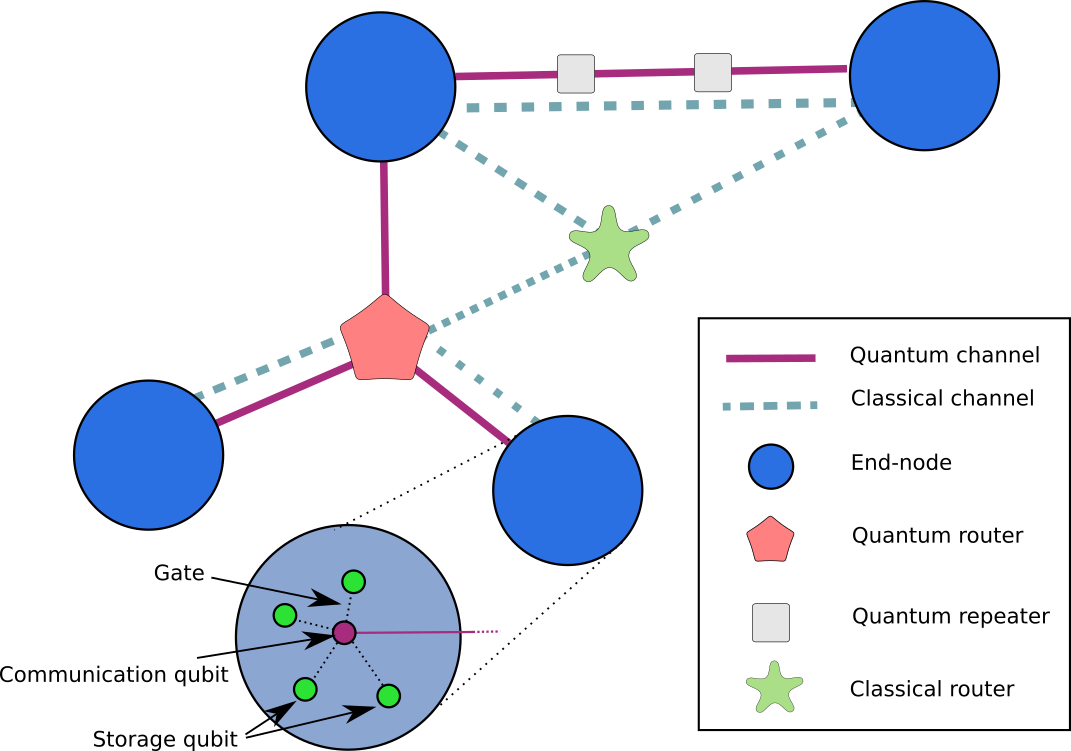
\includegraphics[width=0.4\linewidth]{figures/netqasm/network_model.png}
    \caption{
      Abstract model of a quantum network and its components.
      Quantum network applications run on the \emph{end-nodes} (blue).
      Their communication via classical message passing and quantum entanglement~(\cref{fig:app_programs}) is abstracted away by a network stack.
      That is, it is not visible at the application layer how entanglement generation or classical message passing is realized.
      This may be via direct physical connections, or intermediary repeaters and/or routers.
      End-nodes hold two types of qubits:
        (1) \emph{communication qubits} which can be used to generate entanglement with remote nodes and
        (2) \emph{storage qubits} which can be used to store quantum states and apply operations.
      A communication qubit may also be used as a storage qubit.
      The qubits within an end-node can interact through quantum gates and their state can be measured.
    }
    \label{fig:network_model}
\end{figure}

\subsection{Quantum networks}
\label{sec:quantum_networks}
A schematic overview of quantum networks is given in~\cref{fig:network_model}.
A quantum network consists of \textit{end-nodes} (hereafter also: \textit{nodes}), which contain quantum network processors as well as classical processors.
Nodes are connected by \textit{quantum channels} or \textit{links} that can be used to generate \textit{entangled} quantum states across nodes.
End-nodes possess quantum memory in the form of qubits, which can be manipulated by performing \textit{operations} such as initialization, readout, and single- or multi-qubit \textit{gates}.
Each quantum memory has a certain \textit{topology} that describes which operations can be applied on which (pair of) qubits.
Some of the qubits in a quantum memory may be used to generate an entangled state with another node.
These qubits are called \emph{communication qubits}~\cite{dahlberg2019linklayer}, in contrast to \emph{storage qubits} which can only directly interact with other qubits part of the same local node
\footnote{A storage qubit may however hold a state that is entangled with a qubit in another node: after remote entanglement generation using a communication qubit, the state in that local qubit could be transferred to one of the storage qubits, preserving the remote entanglement.}.

Some platforms only have a single communication qubit and multiple storage qubits~\cite{Bernien2014}, whereas others can have multiple communication qubits~\cite{Inlek2017}.
Qubits are sensitive to \textit{decoherence} and have limited lifetimes.
Therefore, the timing and duration of operations (such as local gates or entanglement generation with another node) have an impact on the quality of quantum memory. Classical processors control the quantum hardware, and also perform classical computation.
Finally, classical links exist between nodes for sending classical messages.

Since end-nodes can control their memory and entanglement generation, they can run arbitrary \textit{user programs}.
End-nodes can both communicate classically and generate entanglement between each other, either directly or through repeaters and routers, (\cref{fig:network_model}). Nodes in the network other than end-nodes, such as repeaters and routers, do not execute user programs; rather these run protocols that are part of some level in the
network stack~\cite{dahlberg2019linklayer,kozlowski2020networklayer}.
These internal nodes in the network perform elementary link generation and entanglement swapping in order to generate long-distance remote entanglement between end-nodes~\cite{dahlberg2019linklayer}.

There are various quantum hardware implementations for quantum network processors, such as nitrogen-vacancy centers in diamond~\cite{Bernien2014}, ion traps~\cite{moehring2007entanglement}, and neutral atoms~\cite{hofmann2012heralded,ritter2012elementary}, which all have different capabilities and gates that can be performed.

In contrast to classical networks, we consider the end-nodes in a quantum network to not have a network interface component that is separated from the main processing unit.
Having local and networking operations combined in a single interface reflects the physical constraint on current and near-term hardware.
Current state-of-the-art hardware for quantum networking devices can make use of up to the order of 10 qubits~\cite{bradley2019solidstate}.
Furthermore, certain hardware implementations, such as nitrogen-vacancy centers in diamond~\cite{Bernien2014}, only have a single communication qubit, which also acts as a mediator for any local gate on the storage qubits.
This prevents dedicating some qubits for purely local operations and some for purely networking operations.
Rather, to make maximal use of near-term quantum hardware, a multi-purpose approach needs to be supported.



\section{Design Considerations and Challenges from QNodeOS (from appendix)}

We start with providing additional information for some of the design considerations and challenges for an operating system for executing applications on a quantum network node.

\subsection{Application Paradigm}

Our architecture is primarily meant to \emph{enable the execution of quantum network applications in the quantum memory stage~\cite{wehner_2018_stages} and above}. That is, applications that require the use of a quantum processor that can manipulate and store quantum bits (qubits). For simpler applications in the prepare-and-measure and entanglement generation stages~\cite{wehner_2018_stages}, e.g. quantum key distribution~\cite{bb84Original,ekert_1991_e91}, where the quantum states are immediately measured by the nodes, our system can also be used, but it would be sufficient to realize a system implementing a quantum network stack and classical processing only.

\paragraph{Separated programs}

Recall that a quantum networking application consists of multiple programs, each running on one of the end nodes, where for ease of explanation we will assume we are executing an application between two nodes, i.e. a client and a server. Each node in the network runs its own independent \emph{\ac{QNodeOS}}, on which the node's program is executed. The two programs may interact with each other via message passing and entanglement generation, where both types of interactions are managed by the node's \ac{QNodeOS}. Next to interaction via the programs, the nodes may exchange additional classical messages which are not part of the program itself, for example, in order to enable the realization of a network stack~\cite{dahlberg_2019_egp} managing entanglement generation between the nodes.

Classical blocks of code consist of instructions for local classical operations and classical message passing. Quantum \emph{blocks of code} consists of
%
\begin{inlinelist}
\item quantum operations (initialization, quantum gates, measurement), 
\item low-level classical control logic (branching on classical variables and loops), as well as 
\item instructions to make entanglement between remote nodes. 
\end{inlinelist}
%
We remark that classical and quantum instructions may require many actions by the underlying \ac{QNodeOS} (and quantum system controlled by it) in order to be fulfilled: it is the goal of such instructions to abstract away aspects of the underlying system.

Classical blocks of code may depend on quantum ones via classical variables generated during the quantum execution (such as measurement results, notification of entanglement generation, and information on the state of the quantum system such as the availability of qubits). Similarly, quantum blocks may depend on variables set by the classical blocks (such as messages received from remote network nodes). Finally, quantum blocks may themselves depend on other quantum blocks via qubits in the quantum memory. 

\paragraph{Performance metrics}

Next to classical metrics, such as utility (see `Methods, Metrics`), throughput or latency~\cite{stankiewicz_commag}, the successful execution of quantum network applications is governed by quantum metrics, which are unique to quantum networks and not present in classical networks. Such quantum network-specific metrics include fidelity (see `Methods, Metrics`), or the probability of success in executing an application, where the latter depends directly on the fidelity of the quantum states prepared.

\paragraph{Mode of Execution}

There exist quantum applications and functionalities, where one pair of programs is executed only once, e.g. a simple example of quantum teleportation~\cite{bennett_1993_teleportation}. As in quantum computing, however, some quantum network applications~\cite{wehner_2018_stages} are expected to succeed only with a specific \emph{probability of success} $p_{\rm succ}$ when executed once. The application is then typically executed many times in succession in order to gather statistics (for example to amplify $p_{\rm succ}$). A common use case for executing the same application repeatedly also occurs when evaluating the performance of a system (as we do here), where the goal is to estimate quantum performance metrics, such as the probability of success or the fidelity (see `Methods, Metrics`).
When executing the same application multiple times, the programmer can choose to launch many instances of the same program at once if multitasking is possible (see below), or to write one program which repeatedly executes the node's part of the program, asking for a successive execution of the application.

\subsection{Interactive Classical-Quantum Execution}

Let us elaborate further on the relation, and differences, between the execution of quantum network applications, and the execution of quantum computing applications: One could envision building a system for executing quantum network applications on top of a simpler system for the execution of quantum computing programs, as long as the latter can be \emph{augmented with networking instructions to generate entanglement}: in essence one quantum block can be seen as one quantum computing program. Such a block may realize mid-circuit measurements by the classical control logic allowed within one quantum block, or error correction. Error correction could in this paradigm be realized both by classical control logic allowed within one quantum block, or by considering the error correction itself as part of the \ac{QDevice} (see \cref{sec:appendix-arch-node_system}) which then only exposes logical qubits and operations to \ac{QNodeOS}, instead of physical qubits and operations. In that sense, one may think of the interactivity required between classical and quantum operations as taking place not only at a higher level, but also stemming from the fact that classical messages are used to create a new interaction between \emph{separate} quantum programs, while in quantum computing we have only one single program.

\subsection{Different Hardware Platforms} 

It is desirable that an architecture for executing quantum network applications is as much as possible platform-independent, specifying a specific \ac{HAL} that allows interfacing with different (quantum) platforms. We consider as a quantum processor system the \ac{QDevice} model (see `Methods, QDevice Model`), exposing a set of physical instructions addressing specific qubits (see~\cref{sec:sec:appendix-qdevice-instructions-operands}). These physical instructions may be dependent on the type of quantum hardware, e.g. NV in diamond, or trapped ions, and
%
\begin{inlinelist}
\item include instructions for initializing and measuring qubits on the chip,
\item moving the state of a qubit to another location in the quantum memory
\item performing quantum gates, as well as
\item to make attempts at entanglement generation at the physical layer~\cite{pompili_2022_experimental}.
\end{inlinelist}

Quantum processors in general offer two types of qubits (see e.g.~\cite{dahlberg_2019_egp}): \emph{communication qubits} which can be used to generate entanglement with remote nodes next to other quantum operations, as well as \emph{storage qubits} which cannot be used to generate entanglement and only for implementing local quantum operations. We remark that on near-term quantum processors, the types of operations also depends on the connectivity of the qubits. That is, not all (pairs of) qubits may allow the same set of quantum operations to be performed on them.

To later enable compile time optimization, it is desirable that quantum hardware furthermore exposes the capabilities of the quantum chip:
%
\begin{inlinelist}
\item the number of qubits,
\item the type of each qubit, 
\item the memory lifetime of the qubits,
\item the physical instructions that can be performed on on the qubit(s) and
\item the average quality of these instructions.
\end{inlinelist}

\subsection{Timescales}

Quantum network programs are meant to be executed between distant nodes, meaning the communication times between them are in the \emph{millisecond} regime. We remark that the same is \emph{not true for networked or distributed quantum computing }: if the goal is to combine several less powerful quantum processors via a network into one more powerful quantum computing cluster, then it is advisable to place the individual processors as close to each other as possible, in order to minimize the time needed to (1) exchange messages, and (2) generate entanglement between processors. Thus, apart from the execution of applications following a different paradigm (see the main part of the paper, \cref{fig:fig1}),
the case of distributed quantum computing also has different timescales than quantum networking. Of course, it is conceivable that in the future, one may also link distant quantum computers into more powerful quantum computing clusters via quantum internet infrastructure.

%\subsection{Scheduling Local and Network Operations}
%\label{sec:sec:design-consid-scheduling}

\subsection{Scheduling Network Operations}

In order for two neighbouring quantum network nodes to produce heralded entanglement between them, they need to simultaneously perform an action to trigger entanglement generation (at the physical layer, \emph{synchronized to nanosecond precision}). This means neighbouring quantum network nodes need to perform a network operation (entanglement generation) in a \emph{very specific} time slot in which they make an attempt to generate entanglement. Such time slots are generally aggregated into larger time bins, corresponding to making batches of attempts in time slots synchronized at the physical layer. We refer to e.g. Ref.~\cite{pompili_2022_experimental} for background information on the physical layer of entanglement generation in quantum networks, and the readers with a background in computer science to e.g. Ref.~\cite{dahlberg_2019_egp} for a detailed explanation of scheduling of entanglement generation in quantum networks.

In short, network operations in quantum networks need to be executed by the node at very specific time bins. These time bins cannot be determined by the quantum node itself. Instead selection of time bins for a specific quantum operation require agreement with the neighbouring node~\cite{dahlberg_2019_egp} (and more generally with the quantum network when the end-to-end entanglement is made via intermediary network nodes) by means of a network schedule, e.g. determined by a (logically) centralized controller, see Ref.~\cite{skrzypczyk_2021_arch}.

\subsection{Scheduling Local Operations versus Scheduling Network Operations}

For computer scientists, we provide further information on the inability to execute at the same time both local as well as networked quantum operations on present-day quantum processors. At a high-level, present-day quantum processor can be seen as both a quantum \ac{CPU}/memory, as well as network device at the same time. Physical properties of the device and its control at the level of experimental physics, prohibits the usage of the quantum processors for both network and \ac{CPU}/memory functions at the same time. A good example is given by the system of \ac{NV} centers in diamond~\cite{kalb_2017_entanglement,humphreys_2018_delivery}: the communication qubit, i.e. the network device, of the \ac{NV} quantum processor system is given by its electron spin. Further storage qubits may be available by the surrounding nuclear spins in the diamond material. However, such nuclear spins cannot easily be addressed without involving the electron spin, prohibiting their use as a separate processor that is independent from the use as a network device. 

It is conceivable that in the future, two devices could be used~\cite{vardoyan_2022_netarch}: one \emph{quantum processor as a network device} (but not as a device for execution of general quantum gates and measurements), and a another \emph{quantum processor performing only local quantum operations} (but not as a device for long-distance networking). The network device could produce entanglement with distant quantum nodes (which may be taking many \emph{milliseconds} to conclude successfully), and only once such entanglement is ready inject it into the second quantum processor. The latter may still involve short-distance entanglement generation between the network device and the second quantum processor, which however is very fast at short distances. This way the time that the second quantum processor would be blocked by networking operations would diminish significantly.

\subsection{Multitasking}

When executing quantum network applications, multitasking is well motivated in order to increase the utility of the system. Multitasking (or time sharing) is a well-established concept in classical operating systems (see e.g.~\cite[Section 1.4]{silberschatz_book_2014}) that allows the concurrent execution of multiple programs. For the reader from physics, we summarize some of these concepts in order to give context, and then reflect on what these imply in our setting.

In order to allow for multitasking, operating systems typically employ a notion of processes (or threads~\cite[Chapter 4]{silberschatz_book_2014}, or tasks~\cite[Section 3.1]{silberschatz_book_2014}), where a process is created whenever a program starts, and the process forms an instance of the program being executed on the system. Multitasking (time sharing) thus refers to the concurrent execution of multiple processes at once, where it is possible to have multiple processes for the same program, corresponding to the execution of several instances of the program in parallel. We remark that the term concurrent thereby refers to the fact that the processes are existing in the system at the same time, while---due to the fact that they need to share limited resources (e.g. a \ac{CPU} or other devices)---not all of them may be running at the same time.

Allowing multitasking requires the system to include a number of additional features:

\subsubsection{Managing Processes}

At a high-level, multitasking requires the system to keep track of the currently running processes, which means that when program starts executing, a process must be registered in the system. Since the system needs to decide which process can be executed at what time, i.e., which process can be given access to the necessary resources to allow its execution, the system needs to keep track of the state of the process, which typically includes
%
\begin{inlinelist}
\item whether it is ready for execution, 
\item currently running, or 
\item whether it cannot currently be executed since it is waiting e.g. for other processes.
\end{inlinelist}

In the case of executing quantum network applications, different parts of the application require different resources in order to run: classical blocks need the classical processor (\ac{CPU}) and potentially network device present in a \ac{CNPU}, while quantum blocks require the quantum processor (\ac{QDevice}). It is desirable for our system that both resources can be used concurrently. That is, two different processes should be able to execute a classical block (on the \ac{CNPU}), and a quantum block (on the \ac{QNPU}) at the same time.

\subsubsection{Memory Management Unit}

A program typically relies on the ability to store classical variables (in a classical memory), as well as quantum variables (the state of qubits in a quantum memory). Such variables are stored in a classical and quantum memory device (here, the quantum processor), respectively. In order to allow multiple concurrent processes at the same time, the system needs to keep track of which part of the classical and quantum memory is assigned to which process. This concept is known broadly as memory management~\cite[Section 1.7]{silberschatz_book_2014} in classical operating systems.

In order to allow multitasking of quantum network applications, we thus require a \ac{QMMU} (next to standard ways of performing classical memory management). The \ac{QMMU} is responsible for the following tasks:

\paragraph{Qubit information handling} 

A \ac{QMMU} has knowledge of the physical qubits available on the underlying quantum hardware, and may keep any other information about said qubits, such as the qubit type (communication or storage qubit) and qubit lifetime. Physical qubits thereby refer to both qubits realized at the device level, e.g. in the electron spin states of the \ac{NV} center in diamond, or at a logical level where quantum error correction~\cite{lidar2013quantum} is used to protect the quantum memory, i.e. one logical qubit is created by performing error-correcting using many device level qubits. A \ac{QMMU} should allow such physical qubits to be assigned to different owners, i.e. different processes, or the operating system itself. 

\paragraph{Transfer of qubit ownership}

The \ac{QMMU} may also allow a transfer of ownership of the qubits from one owner to the other, such as for example from a network process which makes entanglement to a user process. 

\paragraph{Quantum memory virtualization}

A \ac{QMMU} may also provide abstractions familiar to classical computing such as a virtual address space, where the applications refer to virtual qubit addresses that are then translated to physical qubit addresses. This virtual address space avoids the situation in which physical qubit addresses must be bound at compile time, particularly limiting when allowing multiple applications to concurrently run on the same node. This would allow the transparent moving of qubits in a quantum memory in the future (for example moving them from a processor to a memory-only device while the process is waiting, e.g., for a message from a remote node). We remark however that the noise in present-day quantum devices means that any such move introduces a significant amount of additional noise to the quantum state that may prevent the successful execution of the application.

\paragraph{Qubit memory lifetime management}

Advanced forms of a \ac{QMMU} may also cater to the limitations of near term quantum devices, by matching memory lifetime requirements specified by the application code to the capabilities of the underlying qubits, as well their topology, i.e., taking into account which two qubits allow two-qubit gates to be performed on them directly. While one cannot measure the decoherence of a qubit during a general program execution on the quantum level, the \ac{QMMU} could also take into account additional information from the classical control system to signal to the application that a qubit has become invalid.

\subsubsection{Scheduler}

When multitasking, we need to decide which process should be executed at what time. This concept is referred to as  scheduling in classical operating systems~\cite[Section 2.4]{tanenbaum_operating_2005},~\cite[Section 3.2]{silberschatz_book_2014}. We first discuss design considerations for scheduling when executing quantum network applications, and then reflect on how scheduling may be realized at different levels of the operating system for the quantum network nodes. 

\paragraph{General considerations}

We first provide three general considerations for completeness, which are not specific to the execution of quantum network applications but apply to all system in which several resources (such as the \ac{QDevice} and a classical \ac{CPU}) can be used (largely) independently of each other:
%
\begin{enumerate}
\item \emph{Local quantum computation}: in addition to quantum networking, a node's resources must also be reserved for local quantum gates, which are integral parts of quantum network applications.
\item \emph{Multitasking}: for a node to be shared by multiple users, the scheduler should not allocate all the available resources to a single application indefinitely, and instead it should be aware of the presence of multiple applications.
\item \emph{Inter-block dependencies}: quantum and classical processing blocks of an application may depend on results originating from other blocks, and thus cannot be scheduled independently.
\end{enumerate}

\paragraph{Quantum network considerations}

Two specific considerations stand out in the domain of quantum networking:
%
\begin{enumerate}
\item \emph{Synchronized network schedule}: due to the bilateral nature of entanglement, each node needs to have its quantum networking activity synchronized with its immediate neighbors. This means that while the scheduler at each \ac{QNodeOS} node runs independently of each other, nodes must take into account the network schedule which defines when the node needs to perform networking actions with its neighbouring node. 
\item \emph{Limited memory lifetimes}: the performance of quantum networking applications depends on both classical as well as quantum metrics. Once qubits are initialized, or entanglement has been created, the limited lifetime of present-day quantum memories implies that execution must be completed by a specific time in order to achieve a desired level of quantum performance. 
\end{enumerate}

\paragraph{Quantum/classical performance metrics trade-off}

The best quantum performance is reached when the entire quantum network system (all nodes) are reserved for the execution of one single quantum network application. That is, programs are executed in a serial fashion and no multitasking is performed that could introduce delays which negatively impact the quantum performance. However, this approach does not in general achieve the best utilization of the system. 

While our implementation makes use of a simple priority based scheduler, we remark that our work opens the door to apply more advanced forms of schedulers in the future. In particular, the fact that execution quality degrades over time suggests using forms of real-time schedulers for quantum network applications (taking inspiration from the extensive work on this topic in classical systems, see e.g. Ref.~\cite{liu_1973_scheduling}).  We remark that a programmer (or compiler) could provide advise on such (soft) deadlines, for example in the form of a lookup table that includes suggestions for deadlines for a desired level of quantum performance, based on the capabilities provides by the underlying hardware systems (e.g. memory lifetimes, expected execution time of quantum blocks), and the network (e.g. rate and quality (fidelity) of the entanglement that can be delivered). This advise could then be used by the scheduler to inform its scheduling decisions.

We remark that determining precise deadlines (e.g. when too much time has elapsed for the qubits to yield a specific probability of success) is in general a computationally expensive procedure, sometimes estimated in practice by a repeated simulation of the execution. It is an interesting open question to find (heuristic) efficient methods to approximate a performance prediction. We remark that there is no way in quantum mechanics to measure the current quality of a qubit or operation during the ongoing execution, and such qualities are determined by performing estimates independently of the program execution itself. Of course, \ac{QNodeOS} could itself engage in such estimates when idling in order to update its knowledge of the capabilities of the quantum hardware.

To allow for potentially time-consuming classical pre- and post-processing, it is natural to apply such deadlines not for the entirety of the application, but for the period between initializing the qubits and terminating the quantum part of the execution. While outside the scope of this work, we remark that this type of scheduling offers to inspire new work in a form of ``quantum soft-real time'' scheduling, where deadlines may occasionally be missed at the expense of reduced application performance (success probability), to maximize the overall (averaged) performance of the system in which
applications are typically executed repeatedly. 

\paragraph{Scheduling at different system levels}

Above we discussed scheduling at the level of processes, corresponding to executions of program instances. A system may realize scheduling at different levels, including
%
\begin{enumerate}
\item \emph{Classical versus quantum processes}: The system may sub-divide processes into classical processes (executing classical code blocks), and quantum user processes (executing quantum code blocks). In this case, these can be scheduled independently (provided inter-dependencies are taken into account). 
\item \emph{Scheduling of quantum blocks}: The system may further sub-divide quantum processes into smaller units to allow different quantum code blocks of the same process to be scheduled independently.
\item \emph{Scheduling of individual operations}: The level of operating systems is not typically concerned with the scheduling of individual operations, which is instead taken care of by the underlying \ac{CPU}. We remark that while we do not envision this type of scheduling to be part of such a system in the future, but rather be relegated to control hardware in a microarchitecture for quantum nodes as e.g. in 
\textcite{fu_2017_microarch}, our current realization of \ac{QNodeOS} achieves a simple form of instruction schedule by populating an instruction queue in software due to the absence of a suitable low-level microarchitecture.
\end{enumerate}




\section{Background and context from Qoala}

\textit{Quantum nodes}.
A quantum internet connects quantum nodes on which quantum programs may be 
executed.
%(Figure~\ref{fig:qoala_location}). 
In their most general form, such nodes
are \textit{processing nodes} that have a quantum memory to store quantum bits (qubits) on which quantum operations (qubit initialization, quantum gates and measurements) can be performed. Pairs of nodes can establish \textit{entanglement} between them over a quantum network. Entanglement is a special property of two qubits (an \emph{entangled pair}), where one qubit is stored in the memory of each node. Nodes can also exchange classical messages (e.g. via dedicated classical links or the internet), where no guarantees are assumed on their message delivery times. 

\textit{Programs}.
A program is a series of instructions to be executed by a node.
Instructions can be categorized into four types: local classical processing, classical message-passing, quantum local processing (quantum operations), and remote entanglement generation.
A program can keep classical variables in a classical memory, and quantum variables (qubits) in the node's quantum memory during the execution.
Multiple programs, each running on their own node, together form an \textit{application} (see~\ref{fig:program_illustration}), e.g. QKD (two programs, one per node),
or secret sharing~\cite{hillery1999quantum} (a program each on many nodes).
Programs may involve asynchronous operations (e.g. a server awaiting entanglement with multiple clients).

\textit{Network schedule}.
A quantum network stack has been proposed~\cite{dahlberg2019link} and implemented~\cite{pompili2022experimental} that turns entanglement generation into a robust service independent of the quantum hardware platform.
Important for the design of an architecture for the execution of quantum internet applications is that in this stack, the nodes will establish a network schedule of time slots in which they will trigger entanglement generation (due to need to synchronize entanglement generation at the physical layer~\cite{dahlberg2019link} at high-precision (ns)).
This means that once entanglement has been requested from the network, the nodes can use only the slots in the network schedule to produce entanglement between them, imposing constraints on the ability to schedule applications. What's more, in present day systems~\cite{pompili2021realization, krutyanskiy2023entanglement} limitations in the physical devices prohibit the execution of local operations while engaging in network operations (entanglement generation), creating further dependencies between the local quantum execution and entanglement generation. 
As the specifics of network scheduling~\cite{network-scheduling, skrzypczyk2021architecture} are not within scope of this paper,
we assume the existence of a \textit{network controller} that takes application demand for entanglement and issues a network schedule to the nodes. 
A schedule consists of sequential time slots, each with a start time and duration, when the node will trigger entanglement generation.
Nodes are not forced to attempt entanglement in corresponding time slots, and can instead choose to do local processing instead.

%\begin{figure}[ht]
%    \centering
    %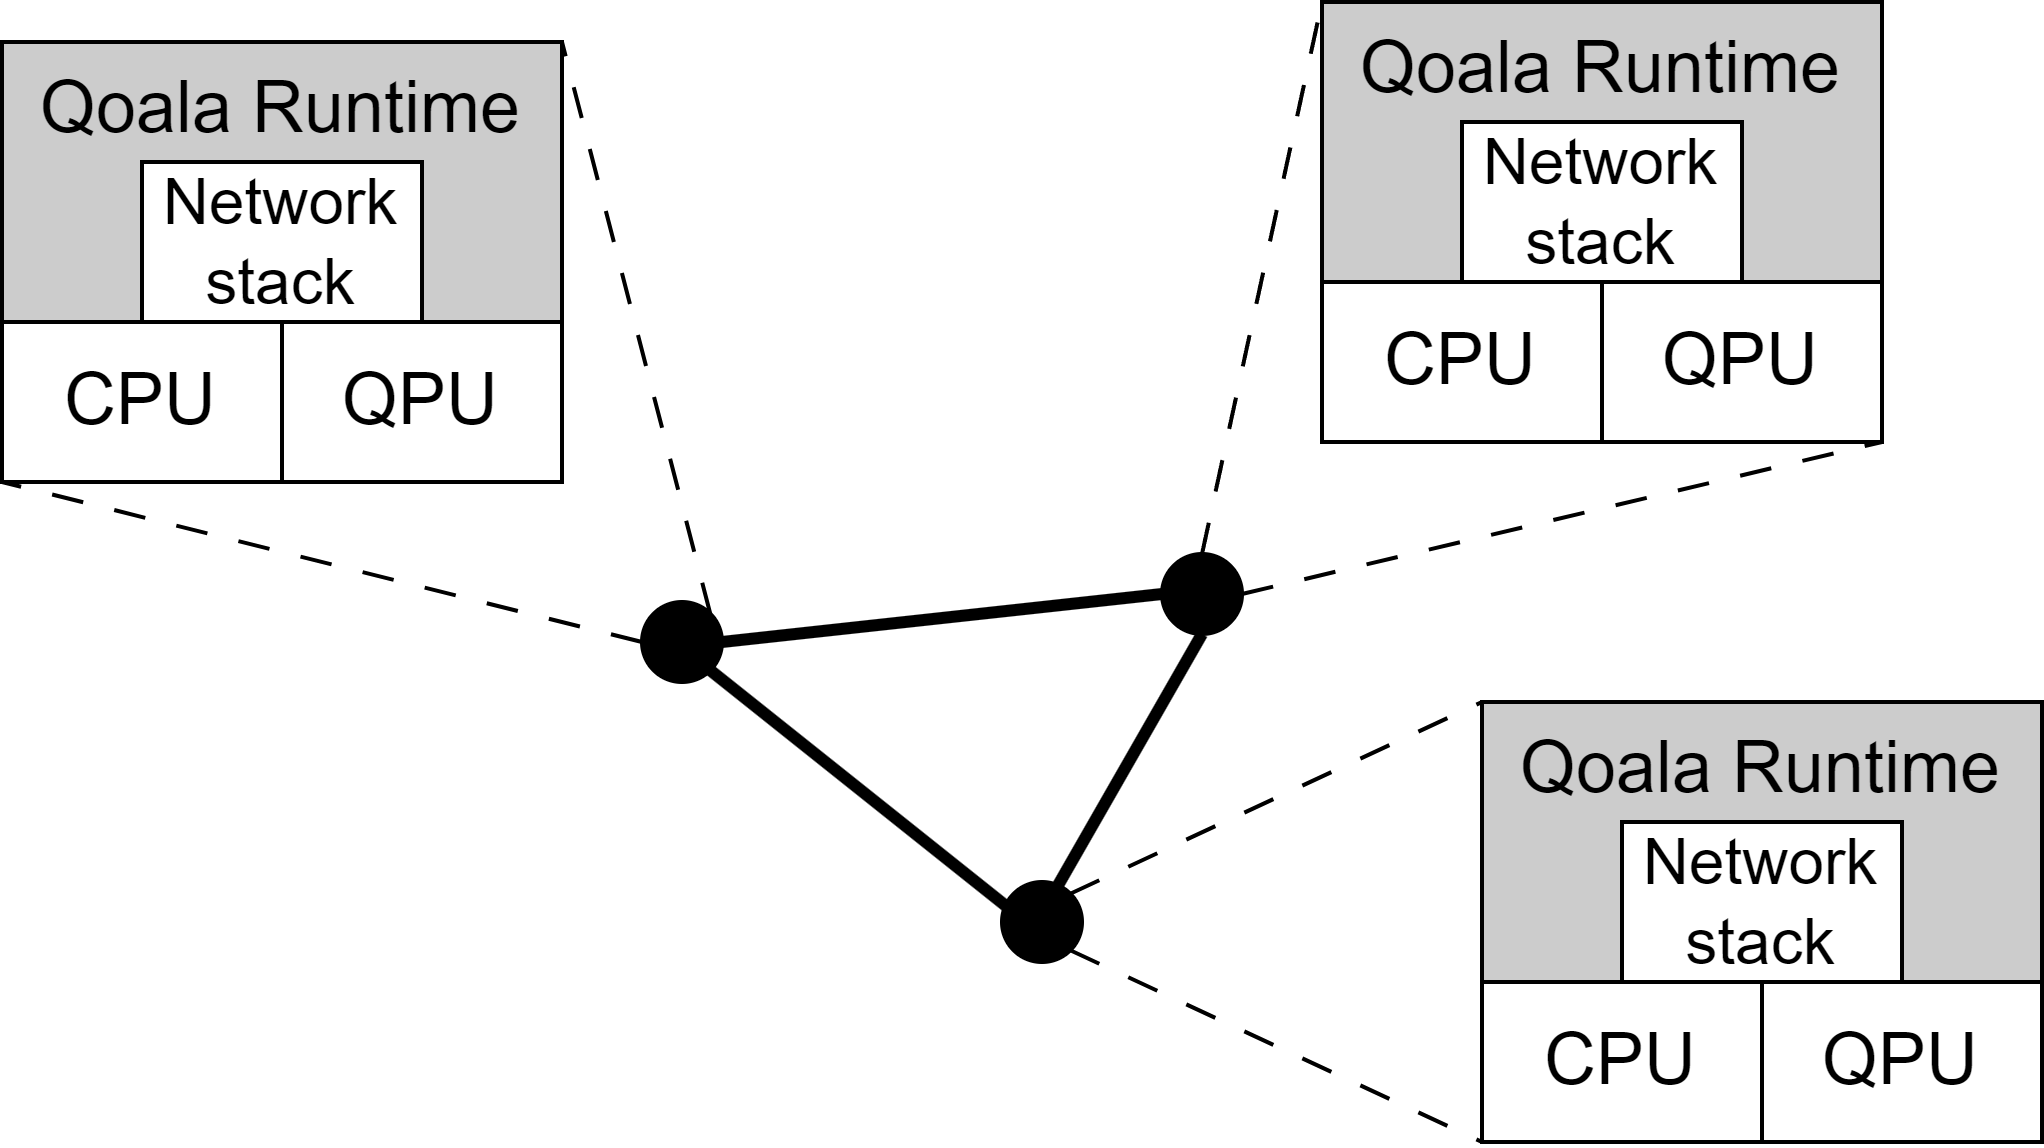
\includegraphics[width=\columnwidth]{figures/qoala/qoala_location.png}
    %\caption{
        %Each node in the quantum internet has its own instance of a Qoala runtime environment, which uses its classical (CPU) and quantum processing (QPU) capabilities, as well as the network stack.
    %}
    %\label{fig:qoala_location}
%\end{figure}

\textit{Performance metrics and noise}. Quantum internet applications have classical outcomes that are typically probabilistic in nature:
(1) applications may intentionally do measurements on quantum states that have fundamentally probabilistic outcomes (e.g. quantum cryptography),
(2) in practice, quantum hardware is imperfect (or \textit{noisy}). That is, undesired errors occur
when performing operations (such as gates, measurements, or entanglement generation) or when keeping quantum states in memory for too long.

In many quantum internet applications (e.g. BQC), a single execution of the application can result in failure or success (e.g. a BQC client receives correct measurement results from the server program~\cite{leichtle2021verifying}). Applications are often executed many times, where outcome statistics are computed in order to validate successful execution (e.g. by majority of outcomes).
We consider two metrics:
a \emph{quantum metric} -  the \textit{success probability} of executing a single instance of the application (on average), and a \emph{classical metric} -  the \textit{makespan}, i.e. the average execution time of an application instance.
